% \textbf{\underline{OZ 4 - De wet van Ampère en de wet van Biot-Savart - Oefening 4:}}
% \vspace{0.5cm}

% Een sfeer met straal $ R $ heeft een uniforme ladingsdichtheid $ \rho $, zoals afgebeeld in Figuur 4.4. Bepaal het magnetisch veld in het centrum van de sfeer wanneer deze roteert als een star object met hoeksnelheid $ \omega $ rond zijn as.

% \begin{figure}[H]
%     \centering
%     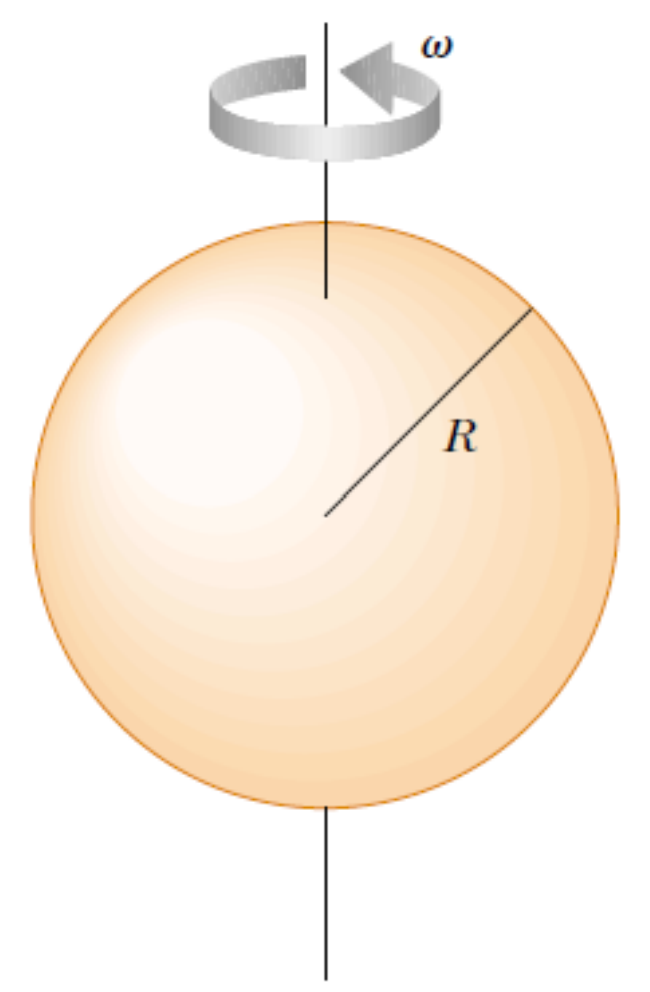
\includegraphics[width=3cm]{oz04/resources/oef-4-opgave.png}
    
%     \textbf{Figuur 4.4}
% \end{figure}

% \begin{description}[labelwidth=1.5cm, leftmargin=!]
%     \item[Geg. :]   $ R $; $ \omega $;
% \end{description}